\documentclass[tikz,dvipsnames,convert={density=300,size=1080x800,outext=.png}]{standalone}
\usepackage{tikz-feynman}

\begin{document}


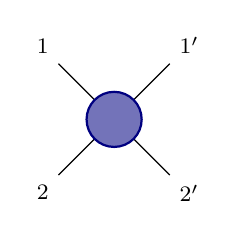
\begin{tikzpicture}
        \begin{feynman}
            \vertex (a);
            \vertex[above left = 0.35cm of a] (h1);
            \vertex[above right = 0.35cm of a] (h2);    
            \vertex[below left = 0.35cm of a] (g1);
            \vertex[below right = 0.35cm of a] (g2); 
            \vertex[above left = 0.65cm of h1, label=above left:{\footnotesize{\(1\)}}] (i1);
            \vertex[above right = 0.65cm of h2, label=above right:{\footnotesize{\(1'\)}}] (i2);    
            \vertex[below left = 0.65cm of g1, label=below left:{\footnotesize{\(2\)}}] (f1);
            \vertex[below right = 0.65cm of g2,label=below right:{\footnotesize{\(2'\)}}] (f2); 
            \diagram*{(i1) -- (h1),
                     (h2) -- (i2),
                     (g2) -- (f2),
                     (f1) -- (g1)};
            \fill[NavyBlue!55] (a) circle (0.35cm) ;
            \draw[NavyBlue,thick]  (a) circle (0.35cm) ;
        \end{feynman}
    \end{tikzpicture}
        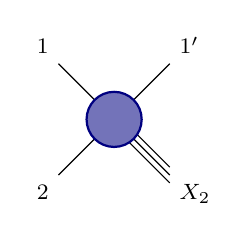
\begin{tikzpicture}
            \begin{feynman}
                \vertex (a);
                \vertex[above left = 0.35cm of a] (h1);
                \vertex[above right = 0.35cm of a] (h2);    
                \vertex[below left = 0.35cm of a] (g1);
                \vertex[below right = 0.35cm of a] (g2); 
                \vertex[above left = 0.65cm of h1, label=above left:{\footnotesize{\(1\)}}] (i1);
                \vertex[above right = 0.65cm of h2, label=above right:{\footnotesize{\(1'\)}}] (i2);    
                \vertex[below left = 0.65cm of g1, label=below left:{\footnotesize{\(2\)}}] (f1);
                \vertex[below right = 0.65cm of g2,label=below right:{\footnotesize{\(X_2\)}}] (f2); 
                \vertex[below = 0.1cm of f2] (f3); 
                \vertex[below = 0.1cm of g2, left = 0.1cm of g2] (g3); 
                \vertex[above = 0.1cm of f2] (f4); 
                \vertex[above = 0.1cm of g2] (g4); 
                \diagram*{(i1) -- (h1),
                         (h2) -- (i2),
                         (g2) -- (f2),
                         (g3) -- (f3),
                         (g4) -- (f4),
                         (f1) -- (g1)};
                \fill[NavyBlue!55] (a) circle (0.35cm) ;
                \draw[NavyBlue,thick]  (a) circle (0.35cm) ;
            \end{feynman}
        \end{tikzpicture}
        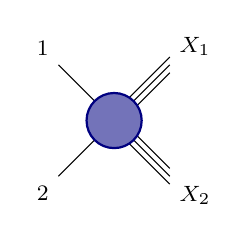
\begin{tikzpicture}
            \begin{feynman}
                \vertex (a);
                \vertex[above left = 0.35cm of a] (h1);
                \vertex[above right = 0.35cm of a] (h2);    
                \vertex[below left = 0.35cm of a] (g1);
                \vertex[below right = 0.35cm of a] (g2); 
                \vertex[above left = 0.65cm of h1, label=above left:{\footnotesize{\(1\)}}] (i1);
                \vertex[above right = 0.65cm of h2, label=above right:{\footnotesize{\(X_1\)}}] (i2);    
                \vertex[below left = 0.65cm of g1, label=below left:{\footnotesize{\(2\)}}] (f1);
                \vertex[below right = 0.65cm of g2,label=below right:{\footnotesize{\(X_2\)}}] (f2); 
                \vertex[below = 0.1cm of f2] (f3); 
                \vertex[below = 0.1cm of g2, left = 0.1cm of g2] (g3); 
                \vertex[above = 0.1cm of f2] (f4); 
                \vertex[above = 0.1cm of g2] (g4); 
                \vertex[below = 0.1cm of i2] (i3); 
                \vertex[below = 0.1cm of h2] (h3); 
                \vertex[above = 0.1cm of i2] (i4); 
                \vertex[above = 0.1cm of h2, left = 0.1cm of h2] (h4); 
                \diagram*{(i1) -- (h1),
                         (h2) -- (i2),
                         (g2) -- (f2),
                         (g3) -- (f3),
                         (g4) -- (f4),
                         (h3) -- (i3),
                         (h4) -- (i4),
                         (f1) -- (g1)};
                \fill[NavyBlue!55] (a) circle (0.35cm) ;
                \draw[NavyBlue,thick]  (a) circle (0.35cm) ;
            \end{feynman}
        \end{tikzpicture}


\end{document}